% !TEX TS-program = pdflatex
% !TEX encoding = UTF-8 Unicode

% This is a simple template for a LaTeX document using the "article" class.
% See "book", "report", "letter" for other types of document.

\documentclass[11pt]{article} % use larger type; default would be 10pt

\usepackage[utf8]{inputenc} % set input encoding (not needed with XeLaTeX)

%%% Examples of Article customizations
% These packages are optional, depending whether you want the features they provide.
% See the LaTeX Companion or other references for full information.

%%% PAGE DIMENSIONS
\usepackage{geometry} % to change the page dimensions
\geometry{a4paper} % or letterpaper (US) or a5paper or....
% \geometry{margin=2in} % for example, change the margins to 2 inches all round
% \geometry{landscape} % set up the page for landscape
%   read geometry.pdf for detailed page layout information

\usepackage{graphicx} % support the \includegraphics command and options

% \usepackage[parfill]{parskip} % Activate to begin paragraphs with an empty line rather than an indent

%%% PACKAGES
\usepackage{booktabs} % for much better looking tables
\usepackage{array} % for better arrays (eg matrices) in maths
%\usepackage{paralist} % very flexible & customisable lists (eg. enumerate/itemize, etc.)
\usepackage{verbatim} % adds environment for commenting out blocks of text & for better verbatim
\usepackage{subfig} % make it possible to include more than one captioned figure/table in a single float
% These packages are all incorporated in the memoir class to one degree or another...

%%% HEADERS & FOOTERS
\usepackage{fancyhdr} % This should be set AFTER setting up the page geometry
\pagestyle{fancy} % options: empty , plain , fancy
\renewcommand{\headrulewidth}{0pt} % customise the layout...
\lhead{}\chead{}\rhead{}
\lfoot{}\cfoot{\thepage}\rfoot{}

%%% SECTION TITLE APPEARANCE
\usepackage{sectsty}
\allsectionsfont{\sffamily\mdseries\upshape} % (See the fntguide.pdf for font help)
% (This matches ConTeXt defaults)

%%% ToC (table of contents) APPEARANCE
\usepackage[nottoc,notlof,notlot]{tocbibind} % Put the bibliography in the ToC
\usepackage[titles,subfigure]{tocloft} % Alter the style of the Table of Contents
\renewcommand{\cftsecfont}{\rmfamily\mdseries\upshape}
\renewcommand{\cftsecpagefont}{\rmfamily\mdseries\upshape} % No bold!

%%% END Article customizations
\usepackage{url}
\usepackage[spanish]{babel}
\usepackage{listings} 
%%% The "real" document content comes below...

\title{BUSCAMINAS PARA ANDROID}
%\date{} % Activate to display a given date or no date (if empty),
         % otherwise the current date is printed 
         
\author{Edinson Sanchez\\Kevin Filella\\Adrian Aguilar}

\begin{document}
\maketitle

%----------------------------------------------------------------------------------------
%	TABLE OF CONTENTS
%----------------------------------------------------------------------------------------

%\setcounter{tocdepth}{1} % Uncomment this line if you don't want subsections listed in the ToC

\newpage
\tableofcontents
\newpage

\section{Introducción}
Buscaminas es un popular video juego, el cual lo podemos descargar y jugar en practicamente todas las plataformas que existen.
El objetivo del juego es limpiar un campo abstracto sin detonar las minas. Normalmente el campo se representa como una matriz cuadrada, aunque debido a la popularidad del juego se han desarrollado
muchisimas variantes en el diseño original del juego.
Imagenes tomadas de wikipedia
diseño en cubo tridimensional y diseño con muhcas minas por posicion

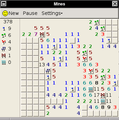
\includegraphics[height=5cm]{imagenes/119px-Firefox_Multiple_mines.png}
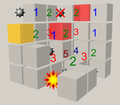
\includegraphics[height=5cm]{imagenes/120px-Cube_Minesweeper_3D.png}
%\includegraphics[height=5cm]{imagenes/File-Xbomb_triangles.png}
\subsection{Objetivo}
Nuestro objetivo en este proyecto es realizar una fiel implementacion del popular juego Buscaminas para sistemas Operativos Android.
Sabemos tambien que la competencia en el mercado es amplia por lo cual debemos , ademas de implementar fielmente las funcionalidades del buscaminas de windows, darle un toque personal y diferente  la presentacion del juego

\section{Desarrollo}
\subsection{Desarrollo inicial}
Inicialmente debido  a la naturaleza del proyecto y a las caracteristicas del curso presente tuvimos que aprender a instalar y manejar las herraminetas de desarrollo adecuadas. Ademas de aprender desde 0 a programar en Android. Con la ventaja de que su entorno de desarrollo default ofrece una IDE mastante amigable al usuario y su lenguaje de programacion es parecido al Java. 


\includegraphics[height=5cm]{imagenes/Android_robot.png}
\section{PROBLEMAS }


\subsection{primer problema}

Durante los primeros pasos en el desarrollo de la aplicacion no tuvimos inconvenientes reales. El parecido con el lenguaje de java hizo que facilemente implementasemos los menus y las pantallas de presentacion
Lo mas dificil de la presentacion y que nos tuvo discutiendo hasta el final fue que clase de botones o celdas utilizariamos para el buscaminas. Button, ToogleButton, ImageButton etc...

\section{Tutorial de Instalación}
\subsection{Debemos ir al siguiente link (http://www.gnu.org/software/mit-scheme/) y descargar el paquete de instalación del lenguaje SCHEME correspondiente al sistema operativo en la q se va a trabajar, en este caso yo instalare el paquete de Windows 7.
lo elegimos e inmediatamente comenzara la descarga del paquete de instalación}
\begin{center}
%\includegraphics[width=12cm]{imagenes/1.png}
\end{center}

\subsection{Ejecutamos el paquete de instalación de SCHEME y aparecerá la siguiente ventana donde le damos en NEXT}
\begin{center}
%\includegraphics[width=12cm]{imagenes/2.png}
\end{center}

\subsection{Ahora nos aparecerá una nueva ventana donde estarán los términos de licencia del programa, si está de acuerdo le da clic en  I AGREE, caso contrario atrás o cancelar}
\begin{center}
%\includegraphics[width=12cm]{imagenes/3.png}
\end{center}

\subsection{Nos aparecerá otra ventana donde debemos ingresar una dirección e el disco duro donde queremos q el programa se instale, si quiere puede dejar la dirección que se encuentra escrita por defecto y le da clic en NEXT}
\begin{center}
%\includegraphics[width=12cm]{imagenes/4.png}
\end{center}

\subsection{Aparecerá una nueva ventana donde podemos cambiar el nombre a la carpeta donde se va a instalar el programa, si quieren pueden dejar el nombre que se encuentra por defecto y dar clic en  INSTALL }
\begin{center}
%\includegraphics[width=12cm]{imagenes/5.png}
\end{center}

\subsection{Comenzara a instalarse el programa hasta que la barra llegue al 100 y aparecerá una nueva ventana donde le damos clic en FINISH para confirmar que el programa se ha instalado correctamente}
\begin{center}
%\includegraphics[width=12cm]{imagenes/6.png}
\end{center}

\subsection{Ahora vemos en nuestro escritorio y nos va a aparecer un nuevo icono que le pertenece al programa SCHEME recién instalado, le damos doble clic y se abrirá}
\begin{center}
%\includegraphics[width=12cm]{imagenes/7.png}
\end{center}

\subsection{Finalmente tenemos instalado en nuestro ordenador el lenguaje SCHEME listo para trabajar}
\begin{center}
%\includegraphics[width=12cm]{imagenes/8.png}
\end{center}

\section{Hola Mundo y otros Programas Introductorios}

% Set your language (you can change the language for each code-block optionally)
\begin{lstlisting}[frame=single]  % Start your code-block
for i:=maxint to 0 do
> (display "Hola mundo")
Hola mundo
\end{lstlisting}
'display' se utiliza para mostrar texto en pantalla. Este código muestra 'Hola mundo' en pantalla.

\begin{lstlisting}[frame=single]  % Start your code-block
for i:=maxint to 0 do
> (sin 90)
1
\end{lstlisting}
Este código muestra el seno de 90 grados en pantalla: 1.

\begin{lstlisting}[frame=single]  % Start your code-block
for i:=maxint to 0 do
> (map + '(5 2 1) '(3 4 4))
(8 6 5)
\end{lstlisting}
'map' recibe un procedimiento y lo utiliza en los elementos de una lista, retornando una lista de resultados.
En este caso, utiliza el operador suma y retorna la suma de las dos listas: (8 6 5).

\begin{lstlisting}[frame=single]  % Start your code-block
for i:=maxint to 0 do
> (define (cuadrado x) (* x x))
> (cuadrado 10)
100
\end{lstlisting}
En este código, hemos declarado una función llamada 'cuadrado' que recibe un parámetro 'x'. El cuerpo de tal función esta después de su declaración, y consiste en elevar 'x' al cuadrado usando el operador de multiplicación. En la siguiente línea, llamamos a la función 'cuadrado' y le enviamos '10' como parámetro, retornando 100 como resultado.
  
\begin{thebibliography}{1}

\bibitem{quote} Gerald Jay Sussman and Guy L. Steele, Jr. {\em The First Report on Scheme Revisited}  December 1998.

\bibitem{url}  WikiBooks - Scheme Programming {\em \url{http://en.wikibooks.org/wiki/Scheme_Programming/}} December 2010.

\end{thebibliography}

\end{document}